
\section{Our Approach}
\label{sec:approach}

In contrast to other systems for accelerating path rendering with GPUs,
our approach {\em explicitly} reveals the coverage determinations.  These
determinations---for both filling and stroking---appear as stencil buffer
updates.
A crucial insight underlying our approach is never determining the
boundary between the ``inside'' and ``outside'' of a stroke or fill.
Instead, we rely on point-sampled determinations of whether a particular
$(x,y)$ framebuffer location is inside or outside the stroke or fill.  For antialiasing, we rely on GPU
multisampling to provide multiple sample coverage positions, each with
its own sub-pixel stencil value.

\subsection{Stencil, then Cover}

We perform path rendering in two steps.  This is not unique; {\em all} path
rendering schemes involve two steps.  The two steps may be ``tessellate,
then render tessellation'' \cite{Direct2D} or ``intersect with scan
line, then paint pixels'' \cite{Rejected} or ``ray cast, then shade''
\cite{Nehab:2008:RRG:1457515.1409088} but each rendering of a path is
inherently sequential in the sense that determining what pixels are
covered must precede shading and blending those pixels.

What is novel in our approach is {\em explicitly} decoupling the two
steps.  We call our approach, with its two decoupled steps, ``Stencil, then Cover'' (StC).
Rather than a single {\tt DrawPath} operation that hides the two-step nature
of path rendering within the implementation, an OpenGL application
using our extension first ``stencils'' the path in the stencil buffer
\cite{Kurt:1995:ieeestyle}, then ``covers'' the path to shade it.

This explicitly decoupled approach has advantages not available
in interfaces that appear to offer a one-step {\tt DrawPath} command.
Our two-step approach makes arbitrary path clipping, mixing with 3D
graphics, programmable blend modes, and other novel path rendering usages
possible.

\subsection{Filling}

\subsubsection{Improvements to Prior Methods}

Our approach to filling paths is inspired by the work of Loop and Blinn
\shortcite{Loop:2005:RIC:1186822.1073303} who developed an efficient fragment
shader-based approach to determining whether or not an $(x,y)$ sample is
inside or outside a given quadratic or cubic B\'{e}zier hull.  In the
Loop-Blinn formulation, inexpensive arithmetic on interpolated texture
coordinates provides a Boolean predicate which when true indicates the
fragment's sample position is not inside the B\'{e}zier region.

Our approach is {\em not} the first time the stencil buffer has been utilized
for stenciling paths.  Kokojima et al. \shortcite{Kokojima:2006:RIR:1179849.1179997} applied
the Loop-Blinn scheme in conjunction with the stencil buffer to
determine the winding number of TrueType glyph outlines.  Kokojima
et al. showed the general filled polygon algorithm of Lane et
al. \shortcite{Lane:1983:AFR:357323.357326}---subsequently popularized for
use with the stencil buffer \cite{RedBook}---can naturally combine with
the Loop-Blinn quadratic discard shader to determine the samples inside
an arbitrarily complex TrueType outline.  After stenciling each glyph
into the stencil buffer, conservative geometry based on a convex hull or
bounding box can test against the non-zero stencil values, shade those
samples, and reset the stencil values back to an initial zero state.

Kokojima's approach does not immediately extend to cubic B\'{e}zier
segments because the inside region within a cubic B\'{e}zier hull is not
necessarily convex.  Rueda et al. \shortcite{Rueda:2008:TSG:1411846.1411922}
addressed this by providing simple topological strategies to subdivide
cubic B\'{e}zier hulls using B\'{e}zier subdivision to guarantee
convexity, but used an overly expensive discard fragment shader based
on B\'{e}zier normalization rather than applying the Loop-Blinn cubic
formulation.

Our approach to handling cubic B\'{e}zier segments builds on all this
work by combining cubic B\'{e}zier convex subdivision rules with the
Loop-Blinn cubic formulation.  We also perform the discard shaders at
sample-rate rather than pixel-rate for improved coverage determinations
and antialiasing. We use interpolation at explicit sample positions and
our target GPU's sample mask functionality to evaluate multiple samples
within a pixel in a single shader instance.

PostScript, SVG, and other standards support partial circular and
elliptical arcs so an additional discard shader, expressed in Cg, handles
these cases:
\label{round-coverage-shader}
%\vspace{-3pt}
\begin{lstlisting}
void roundCoverage(float2 st : TEXCOORD0.CENTROID)
{
  if (st.s*st.s + st.t*st.t > 1) discard;
}
\end{lstlisting}
%\vspace{-1em}
with the $(s,t)$ texture coordinates assigned so (0,0) is centered
at the origin of roundness to discard
samples outside the arc region contained in a sequence of one or more
polygonal hulls bounding such arcs.

\subsubsection{Baked Form of Filled Paths}

In order to render a filled path, we ``bake'' the path into a
resolution-independent representation from which the path can be stenciled
under arbitrary projective transforms.  This baking process takes time
linearly proportional to the number of path commands.  The resulting baked
path data resides completely on the GPU.  The required GPU storage is
also linearly proportional to the number of path commands.  For a static
path, the baking process needs to be done just once; the baking process must
be repeated if the path's commands or coordinates change, but edits to
the path, including insertions and deletions of commands, require just
re-baking the path segments at or immediately adjacent to the edits.

Once baked, a filled path is reduced to five sets of primitives:
%\vspace{-3pt}
\begin{enumerate}
  \item Polygonal anchor geometry (structured as triangle fans), rendered
  with no shader.
  \item Quadratic discard triangles, rendered with a Loop-Blinn quadratic
  discard shader.
  \item Cubic discard triangles (if the cubic B\'{e}zier hull is a
  triangle) and quadrilaterals, rendered with a Loop-Blinn cubic discard
  shader.
  \item Arc discard triangles, rendered with the {\tt roundCoverage}
  discard shader shown above.
  \item Conservative covering geometry, typically a triangle fan or
  quadrilateral.
\end{enumerate}
Primitive sets \#1 through \#4 are rendered during the stencil fill step.  Two-sided stencil testing increments non-discarded stencil samples of front-facing primitives; back-facing primitives instead decrement non-discarded stencil samples.
Primitive set \#5 is rendered during the cover fill step.  Primitive sets
\#2 through \#4 have properly assigned texture coordinates that drive
each set's respective discard shader.  Figure \ref{fig:filling-explained}
visualizes the baked anchor, discard, and cover geometry.

\begin{figure}[tb]
  %\center{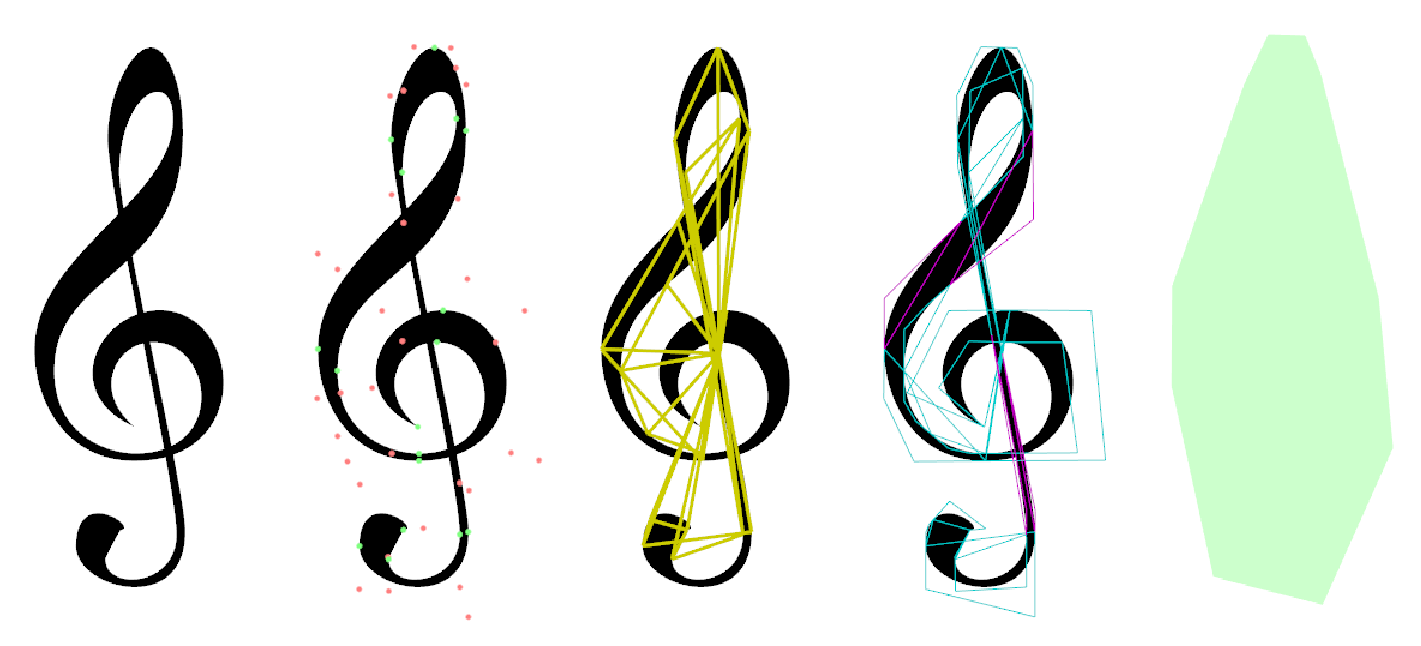
\includegraphics[width=\columnwidth]{filling_explained.eps}}
  \center{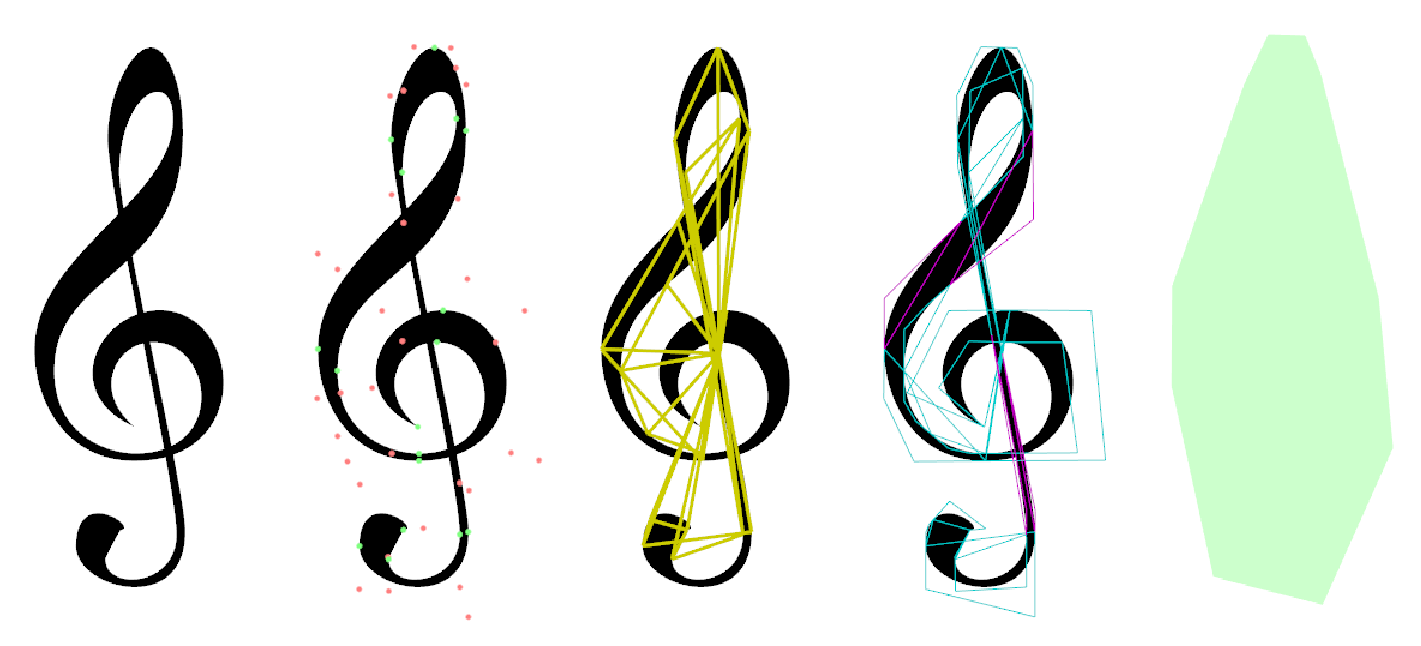
\includegraphics[width=3.3in]{filling_explained.eps}}
  \caption{\label{fig:filling-explained} Filled path, with control
  points, with anchor geometry, and with cubic B\'{e}zier discard hulls,
  and conservative cover geometry.}
\end{figure}
 
This approach to path filling is theoretically sound because the stencil
rendering reduces to a winding number computation consistent with a discrete
formulation of Jordan's Theorem \cite{625138}.

All the data for a baked path can be stored within a single allocation of
GPU memory to minimize the expense of stenciling or covering the path.
Because the baked representation is completely resolution-independent,
robust, and entirely on the GPU, the CPU overhead to launch the stenciling
and/or covering of an already baked path object is minimal.

%By implementing our approach as an OpenGL extension---named {\tt
%NV\_path\_rendering} \cite{NVpr}, performing the stencil and cover steps
%avoids the API and driver validation overhead (explained in
%Section~\ref{sec-performance}) that has plagued other GPU-based approaches
%to path rendering.

We implement our approach as an OpenGL extension named {\tt
NV\_path\_rendering} \cite{NVpr}.  Performing the stencil and cover steps
within the graphics driver avoids
the API and driver validation overhead (see
Section~\ref{sec-performance}) that plagued other GPU-based approaches.
Figure~\ref{fig:pipelines}
shows how our new path pipeline co-exists with the existing pipelines
in OpenGL for pixel and vertex processing.

\begin{figure}[tb]
  %\center{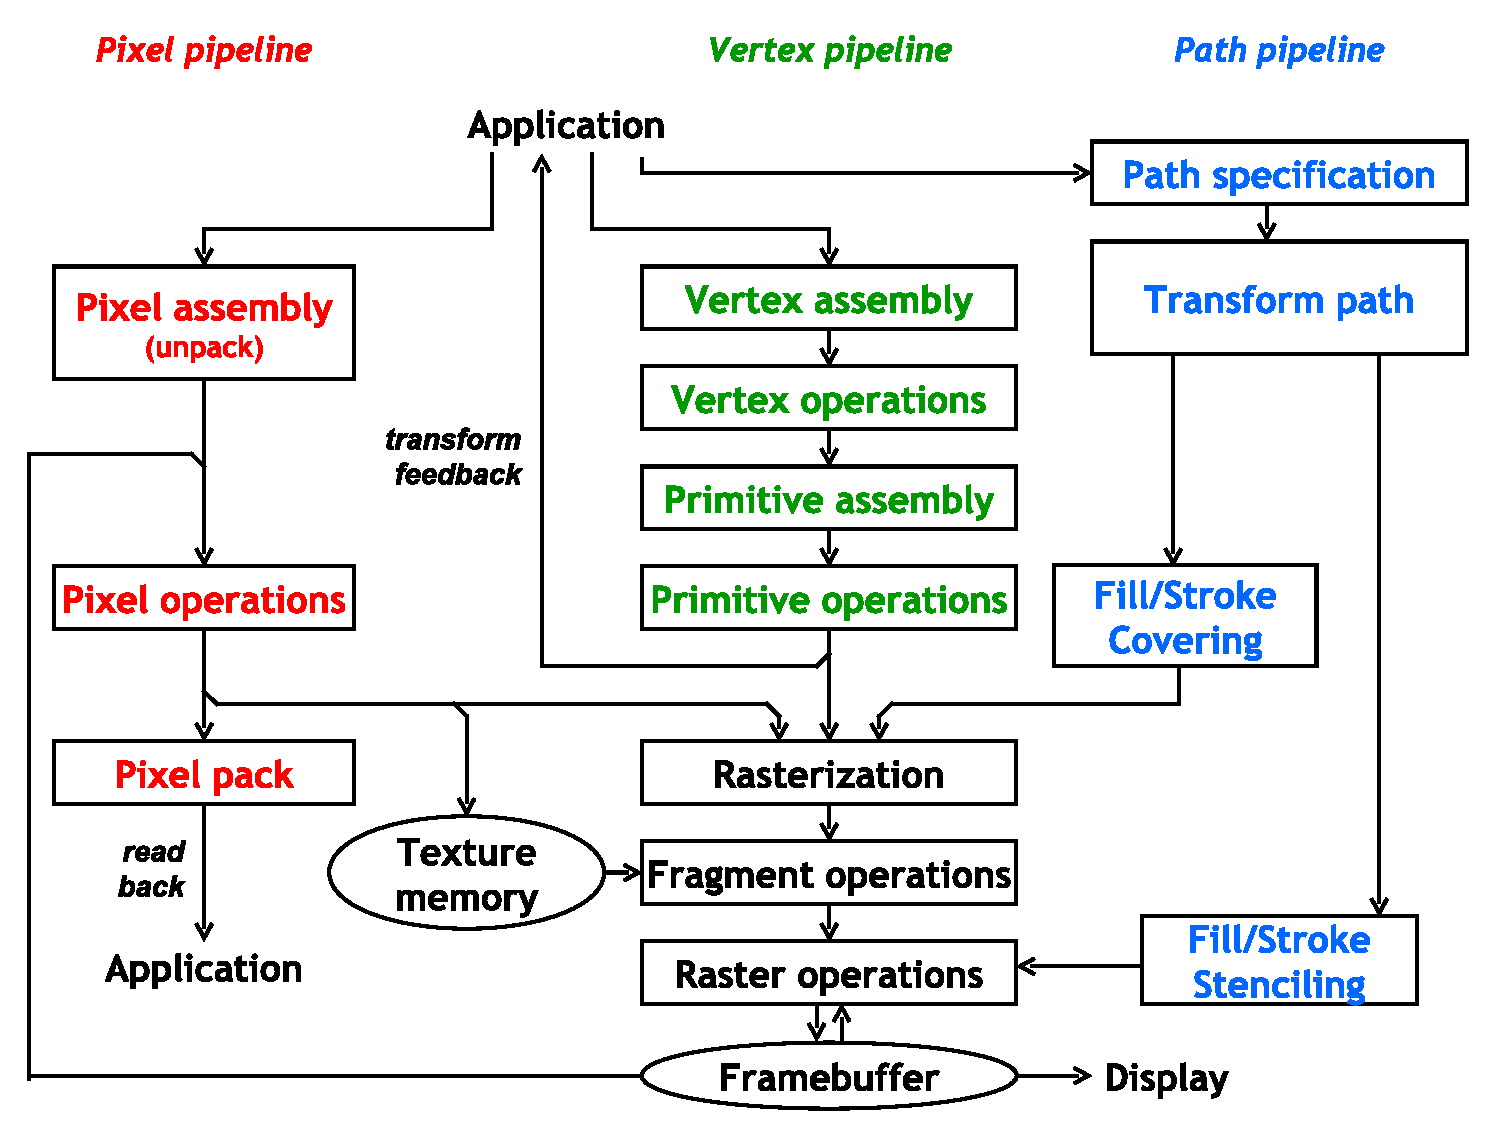
\includegraphics[width=\columnwidth]{pipelines.eps}}
  \center{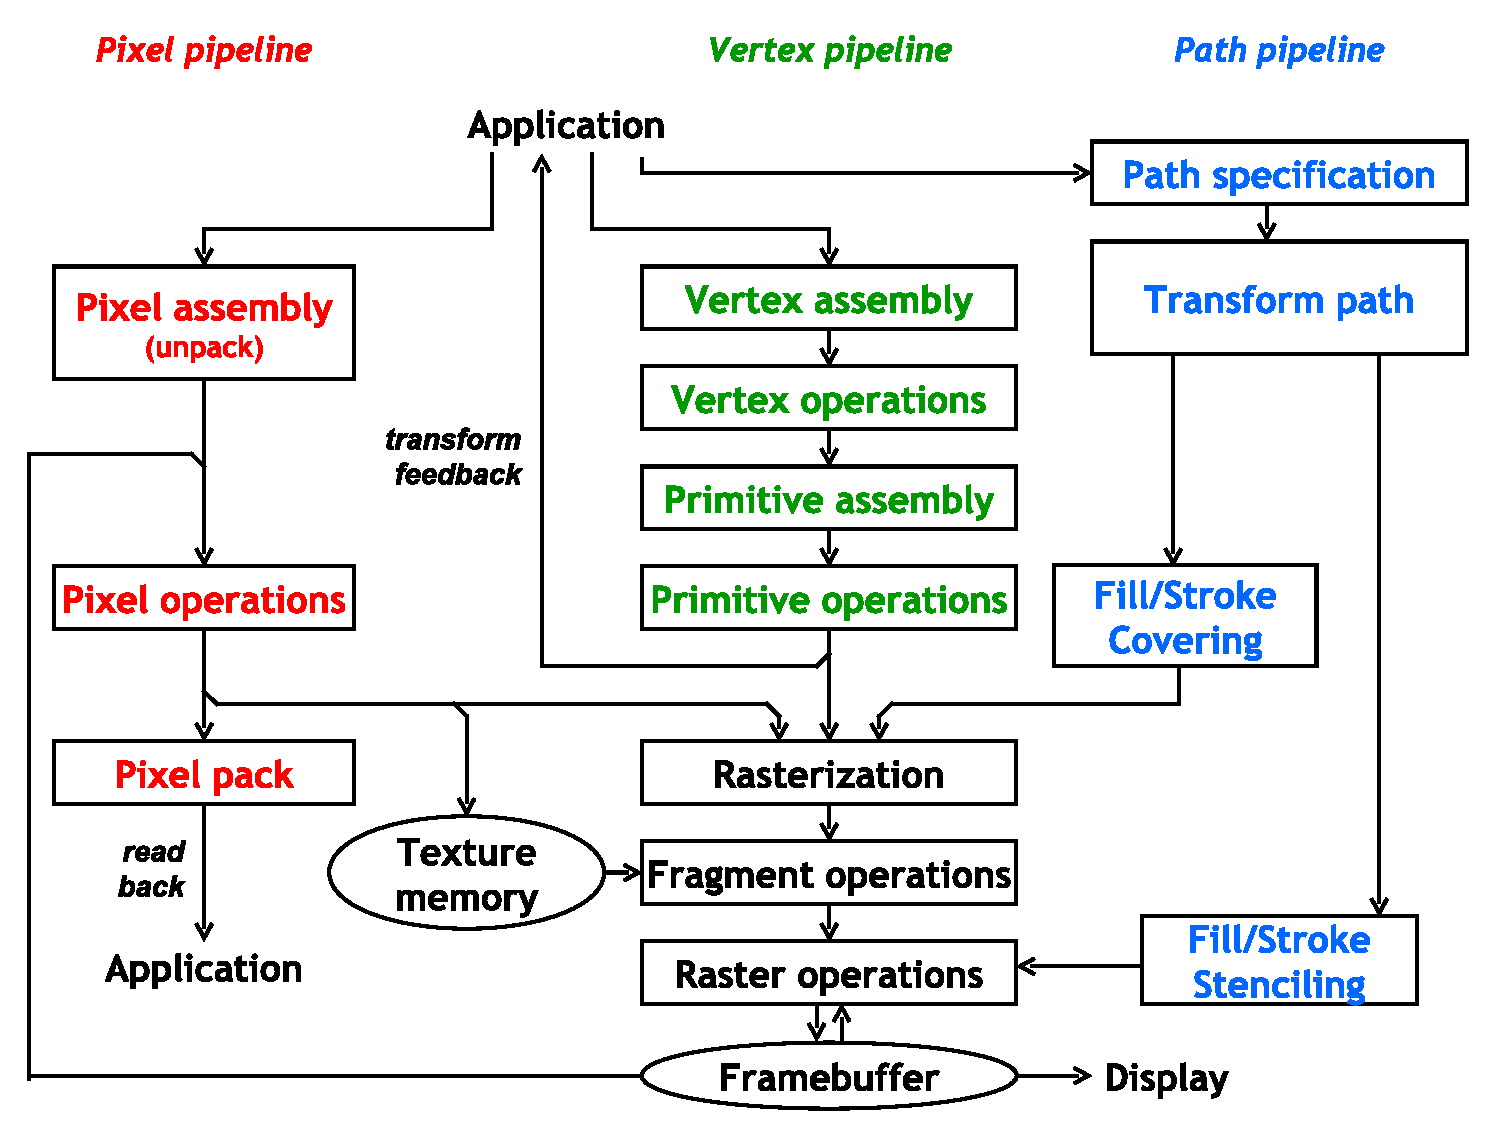
\includegraphics[width=2.8in]{pipelines.eps}}
  \caption{\label{fig:pipelines} High-level data flow of OpenGL showing
  pixel, vertex, and new path pipelines.}
\end{figure}
 
\subsection{Stroking}

Our stroking approach operates similarly to our filling approach whereby
we stencil, then cover stroked paths from a baked resolution-independent
representation residing on the GPU that requires minimal CPU overhead
to both stencil and cover.

\subsubsection{Quadratic B\'{e}zier Stroking}

Analytically determining the points contained by a stroke curved
segment is \underline{not} easy.  The boundary of the stroked region
of a quadratic B\'{e}zier corresponds to an offset curve.  While the
quadratic B\'{e}zier curve generating the offset curve is \nth{2} order,
the offset curve for this generating segment's boundary is \nth{6} order
\cite{Salmon}.  This makes exactly determining an intersection with
this boundary unfeasible, particularly within the execution context
of a GPU's fragment shader.  The boundary becomes even more vexing for
partial elliptical arcs and cubic B\'{e}zier segments.  The boundary for
a general cubic B\'{e}zier curve is \nth{10} order \cite{Farouki1990101}!

\paragraph{Quadratic B\'{e}zier Segment Point Containment}

Hence our approach involves simply determining if a given $(x,y)$ point is
inside or outside the stroked region of a quadratic B\'{e}zier segment.
This can be reduced to solving a \nth{3} order equation.

A quadratic B\'{e}zier segment $Q$---defined by the segment's three
control points $C_0$, $C_1$, and $C_2$---can converted to monomial
form $Q(t)=At^{2}+Bt+C=0$ for $t \in [0,1]$.  A point $P$ is judged
within the stroke of $Q$ when there is a parametric value $s$ on $Q$
such that $Q'(s) \cdot (P-Q(s))=0$ and the squared distance between $Q(s)$ and
$P$ is within the squared stroke radius.  (The dot product of a quadratic
function and the derivative of a quadratic function is \nth{3} order.)
Intuitively this corresponds to finding the 1 or 3 points $Q(s)$ with
a tangent direction orthogonal to the segment connecting $P$ and $Q(s)$.
Such solutions $s$ will be local minima or maxima for the distance between
$P$ and points on $Q$ so computing the squared distance $d=(Q(s)-P) \cdot
(Q(s)-P)$ for each solution $s$ indicates if $P$ is within the stroke of
$Q(t)$ for $t \in [0,1]$ when both $s \in [0,1]$ and $d$ is less than or
equal the square of half the path's stroke width.  Figure~\ref{fig:quadratic-stroke} visualizes this procedure.

\begin{figure}[t]
  %\center{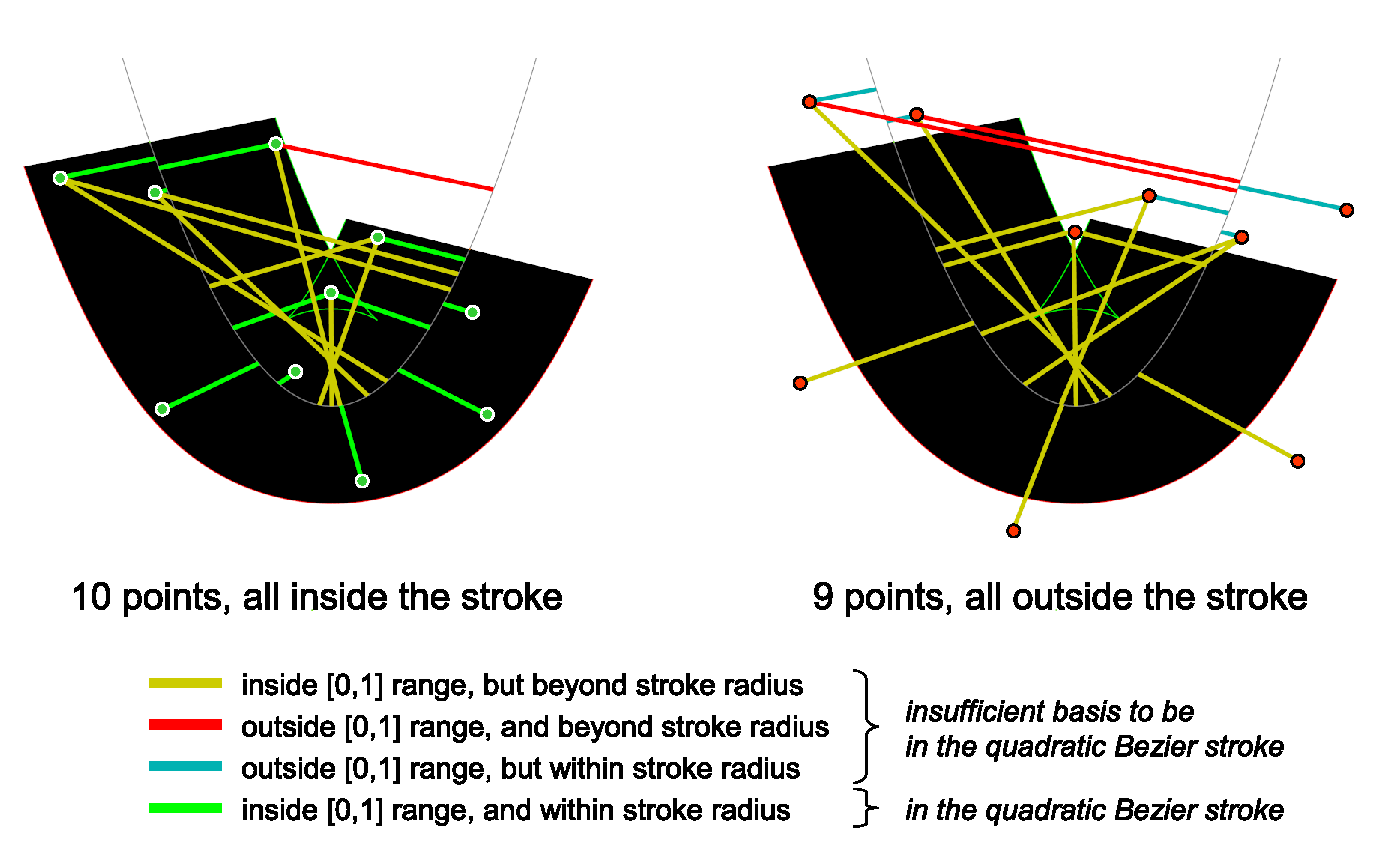
\includegraphics[width=\columnwidth]{quadratic_stroke.eps}}
  \center{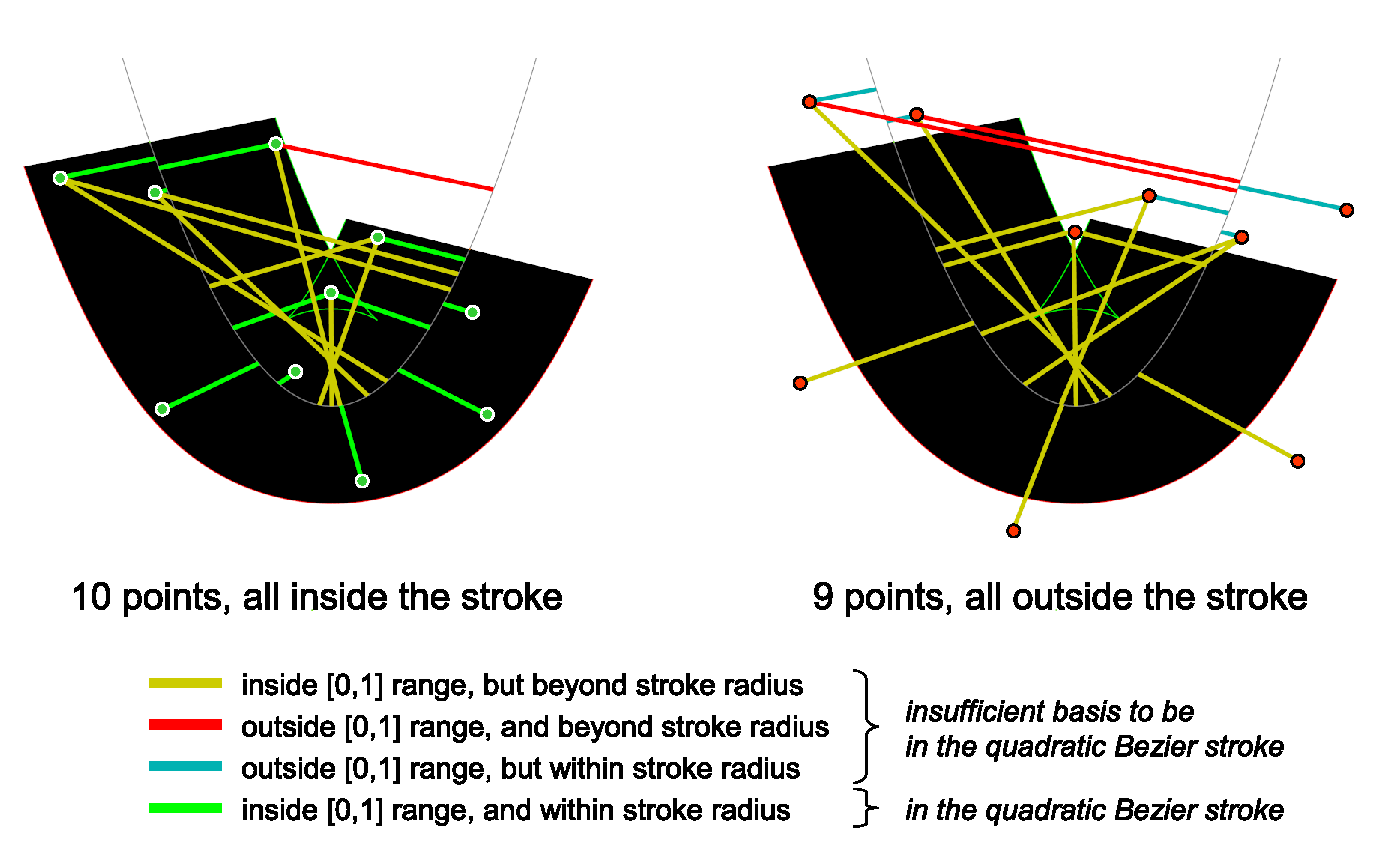
\includegraphics[width=3.3in]{quadratic_stroke.eps}}
  \caption{\label{fig:quadratic-stroke} Visualization of points within
  and outside the stroked region of a quadratic B\'{e}zier segment and
  their basis for inclusion or not.}
\end{figure}

Solving the cubic equation at every rasterized sample is expensive,
but the computation can be simplified somewhat.  The cubic equation can
be rearranged into an easier-to-solve depressed cubic \cite{Cardano} of
the form $t^3+G(x,y)t+H(x,y)=0$.  While the coefficients $G(x,y)$ and $H(x,y)$
are different for every path-space $(x,y)$ location, the functions $G$ and
$H$ are linear in terms of $(x,y)$ so a vertex shader can evaluate $G(x,y)$
and $H(x,y)$ at hull positions and exploit the GPU's ability to interpolate
linearly $G$ and $H$ at positions within the hull.

Care is taken when an arrangement of quadratic B\'{e}zier control points
is collinear, collocated, or very nearly so.  In such cases, we demote
the quadratic B\'{e}zier segment to its linear degenerate equivalent
for robustness.

\begin{figure}[t]
  %\center{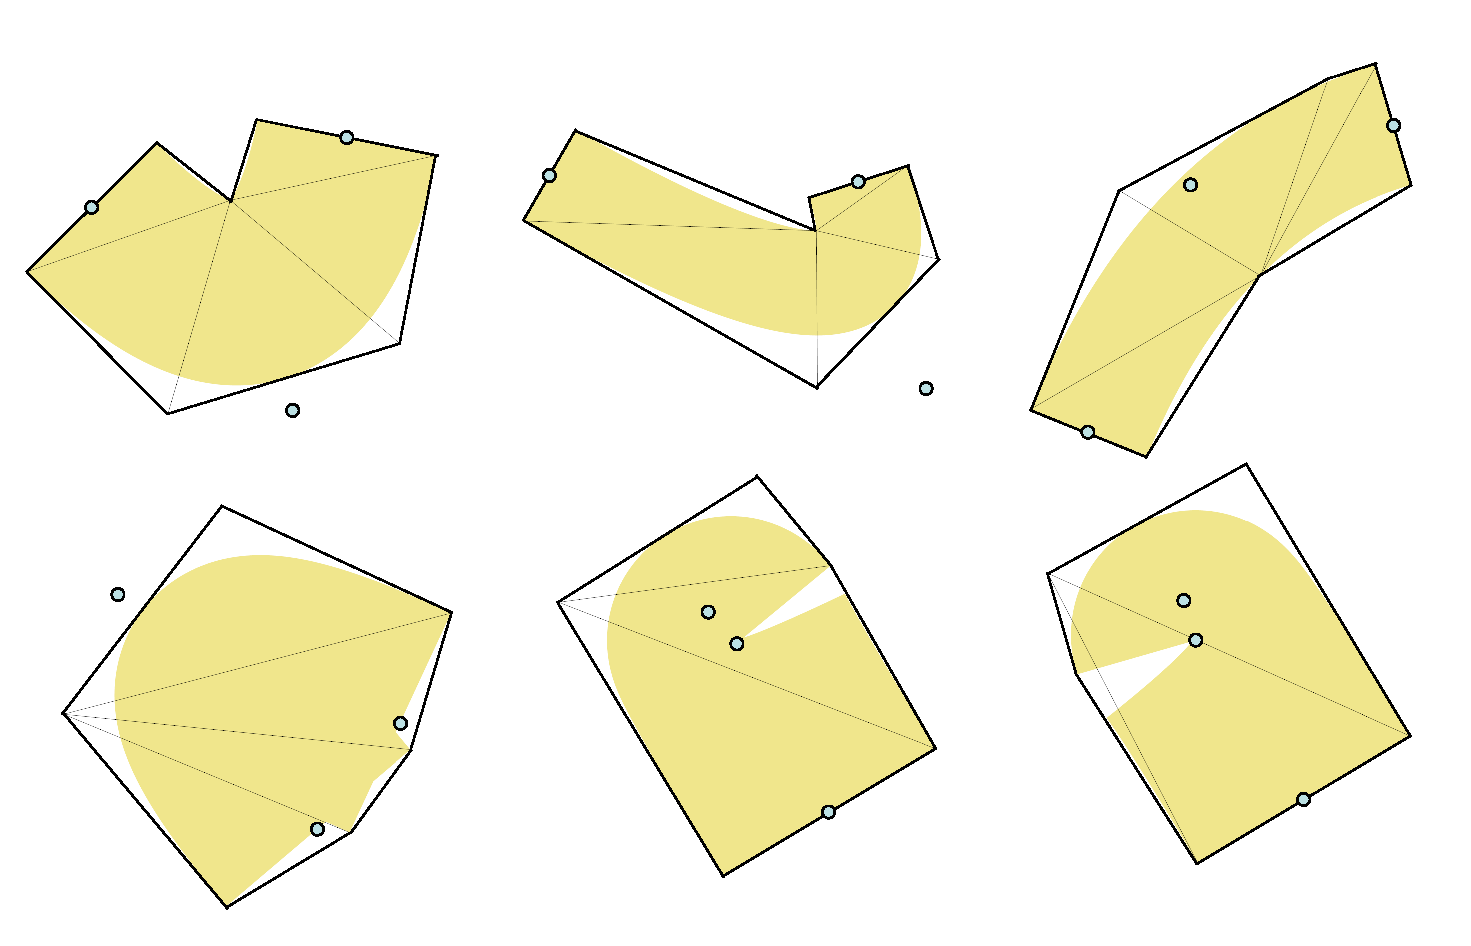
\includegraphics[width=\columnwidth]{quadratic_hull.eps}}
  \center{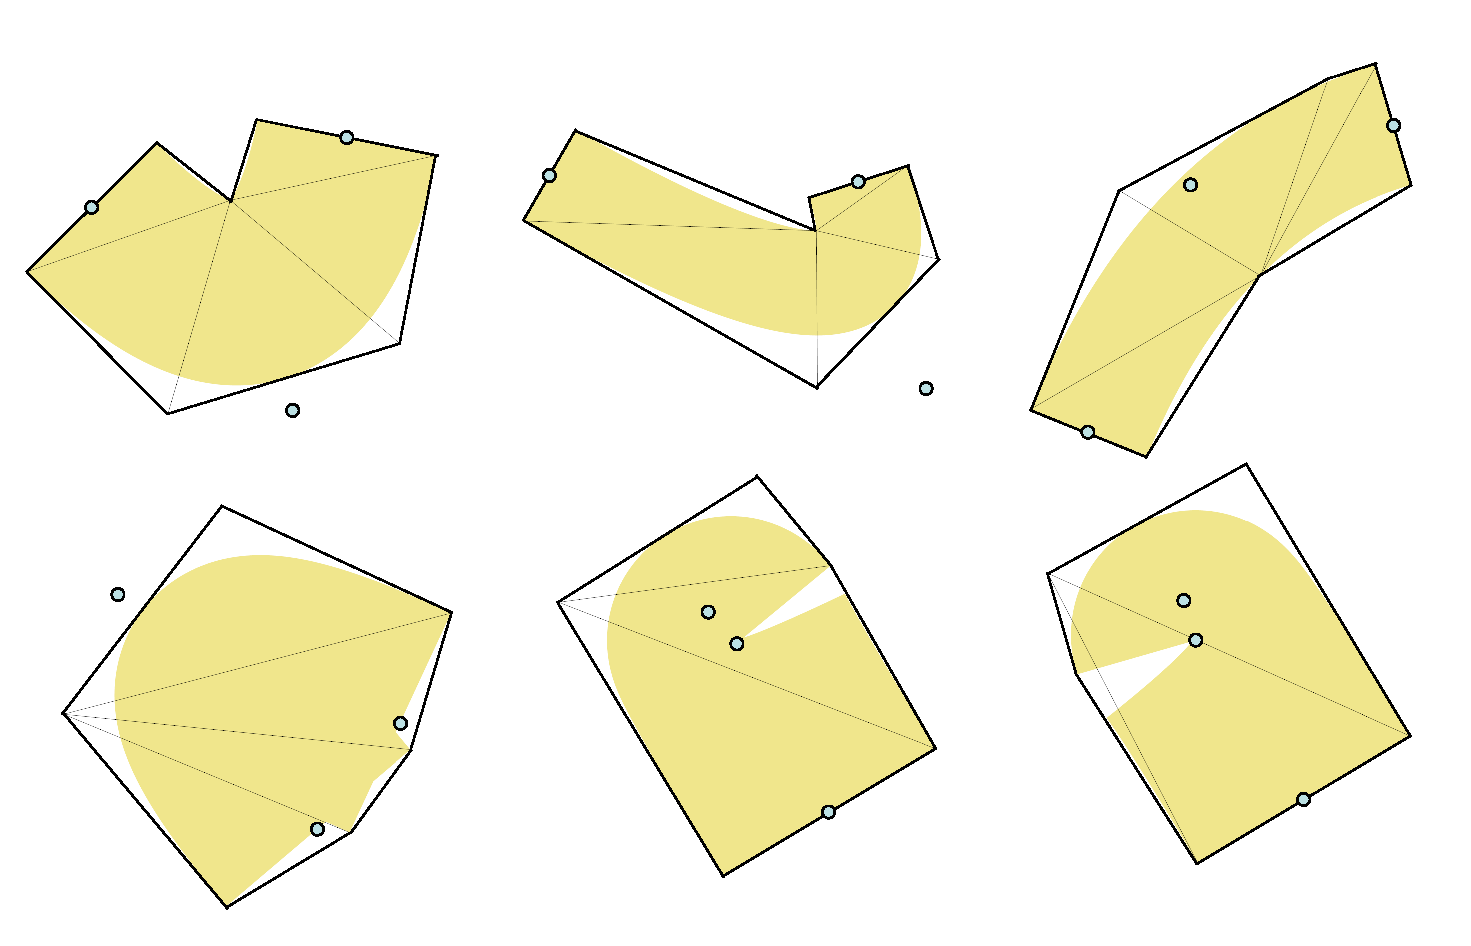
\includegraphics[width=3.3in]{quadratic_hull.eps}}
  \caption{\label{fig:quadratic-hull} Examples of concave (top row)
  and convex (bottom row) stroked quadratic B\'{e}zier segment hulls.}
\end{figure}
 
\paragraph{Stroked Quadratic Segment Hull Construction}

To harness this approach for rendering, we construct a hull
around the quadratic B\'{e}zier stroked segment.  As shown in
Figure \ref{fig:quadratic-hull}, the hull is typically concave,
consisting of seven vertices---though the hull may be convex when
the quadratic stroke's width is wide relative to its arc length.
Ruf \shortcite{Ruf:2011:IBR:2018323.2018346} has addressed the problem of a
tight bounding representation for quadratic strokes, but his approach
involves parabolic edges with the assumption the CPU can evaluate such
edges efficiently; for our purposes, we want a triangular decomposition
of the hull suitable for GPU rasterization.

While solving the cubic equation---even in depressed form---is expensive,
we note that stroked regions are typically small and narrow in screen
space so this expensive process is used sparingly in practice.  Even when
strokes are wide, the massively parallel nature of the GPU makes this
approach quite fast.  Most important to us, once a quadratic stroke
is ``baked'' for rendering, it can be rendered under an arbitrary
linear transformation---including projection---without any further
CPU re-processing.  The hull vertices and their coefficients for $G$
and $H$ can be stored in GPU memory so that stencil-only rendering the
quadratic stroke involves simply configuring the appropriate buffers,
the appropriate vertex and fragment shader pair, and rendering the
hull geometry of the quadratic stroke.

\paragraph{Higher-order-than-Quadratic Stroking}

Path rendering standards incorporate cubic B\'{e}zier segments and
partial elliptical arcs; these involve cubic and rational quadratic
generating curves for rasterized offset curve regions.  The direct
evaluation approach applied to generating quadratic B\'{e}zier curves
is not tractable.

Instead we subdivide cubic B\'{e}zier segments and partial elliptical
arcs into an approximating sequence of quadratic B\'{e}zier segments.
To maintain a curved boundary appearance at all magnifications, our
subdivision approach maintains $G^1$ continuity at quadratic B\'{e}zier
segment boundaries.  No matter how much you zoom into the boundary of
higher-order stroked segments, there is never any sign of linear edges
or even a false discontinuity in the curvature.

Following the approach of Kim and Ahn \shortcite{KimAhn}, we bound the
subdivision such that the true higher-order generating curve never escapes
a specified percentage threshold of the stroke width of the approximating
quadratic stroke sequence.  We also subdivide at key topological features,
specifically points of self-intersection and minimum curvature.

\subsubsection{Stroking Embellishments}

Stroking of line segments, end caps, and joins is straightforward.
Stroked line segments are drawn as stencil-only rectangles.  Polygon
caps (square and triangular) and joins (bevel and miter) are likewise
drawn as stencil-only triangles.  This geometry can be drawn without
any fragment shader.  Round caps and joins are drawn with the same
{\tt roundCoverage} stencil-only sample-rate discard shader (Section
\ref{round-coverage-shader}) used for partial circular and elliptical
arcs for filling with the $(s,t)$ texture coordinates assigned appropriately
to discard samples outside the circular region of the round cap or join.
The baking process for stroked paths includes generating the rectangles
and triangles for line segment and polygonal caps and joins.  Geometry for
round caps and joins is generated along with the texture coordinates to
drive the round coverage discard shader.

\subsubsection{Dashing}

Dashing is a feature of all major path rendering standards except Flash.
Dashing complicates stroking by turning on and off the stroking along
a path based on an application-specified repeating on-off pattern
specified in units of arc length.  Our stroke baking process applies
the dash pattern while gathering the geometry for the stroked path.
While complicated in its details, our dashing process is similar to other
path rendering implementations in its high-level structure.  The primary
difference is curved path segments are reduced to quadratic B\'{e}zier
segments in our approach instead of line segments.  Whereas the arc
length computations in conventional path rendering systems typically
involve recursive subdivision until the curved segment approximates
a line segment, our approach can stop subdividing at
quadratic B\'{e}zier segments.  Unlike higher order curves, the
arc length of a quadratic B\'{e}zier segment (a segment of a parabola)
has a closed form analytical solution:
\begin{eqnarray*}
\lefteqn{ \int _{0}^{1}\!\sqrt {Q_{x}(t)^{2}+ Q_{y}(t)^{2}}{dt} = } \\
&
\frac{\ln ({\frac {b+2\,\sqrt {ac}}{b+2\,c+2\,\sqrt {c\left (c+a+
b\right )}}})\left ({b}^{2}-4\,ac\right )+2\,\left (b+2\,c\right )
\sqrt {c\left (c+a+b\right )}-2\,b\sqrt {ac}}{8c^{3/2}}
\end{eqnarray*}
with copious common subexpressions and 
where $a=B \cdot B$, $b=2B \cdot C$, and $c=C \cdot C$.  Our interest in
this approach is our desire to minimize use of expensive recursive
subdivision algorithms while baking stroked paths, particularly during
dashing.  Some numerical care must be taken to avoid negative square
roots, negative logarithms, and division by zero, but these cases occur
when quadratic segments are nearly linear.
%Using double precision and using Euclidean distance computations when
%control points are collinear---or nearly so---works.

Our dashing approach results in a resolution-independent baked form of
the dashed stroked path.  Once dashed and baked, no further CPU-based
processing is necessary to render dashed paths.  This is in contrast to
other implementations of dashed stroking where dashing has a considerable
CPU processing expense during rendering.  While our implementation must
of course represent each segment resulting from dashing, our render-time
algorithm is completely oblivious to whether the original path was
dashed. 

\subsubsection{Baked Form of Stroked Paths}

Once baked, a stroked path is reduced to four sets of primitives:
%\vspace{-3pt}
\begin{enumerate}
  \item Polygonal geometry (line segments, bevel and miter joins, square
  and triangular end caps) with no shader.
  \item Triangle fans corresponding to quadratic B\'{e}zier segment hulls
  (curved path segments), rendered with a stroked quadratic discard
  shader.
  \item Triangle fans corresponding to round hulls (round end caps and
  joins) rendered with a round coverage shader.
  \item Conservative covering geometry, typically a triangle fan or
  quadrilateral.
\end{enumerate}
Primitive sets \#1 through \#3 are rendered during the stencil stroke
step.  Primitive set \#4 is rendered during the cover stroke step.

The {\tt REPLACE} stencil operation used for stroking is order-invariant.
Therefore we select a static rendering order during the baking process
that minimizes GPU state changes during rendering.

The geometry, texture coordinates, and per-hull quadratic discard shader
coefficients are all packed into a single GPU buffer allocation.  The
rendering process for stenciling the baked path is very straightforward,
requiring no more than three GPU state reconfigurations, one per primitive
set above.

The GPU storage for the linear and quadratic path segments in a
baked stroked path is linearly proportional to the number of segments
(post-dashing).  For cubic B\'{e}zier segments and partial elliptical
arcs, the storage depends on their required level of subdivision.
Because this subdivision is tied to the stroke width, narrower stroke
widths require more storage while wider stroke widths require less
storage.
 
\begin{figure}[tb]
  %\center{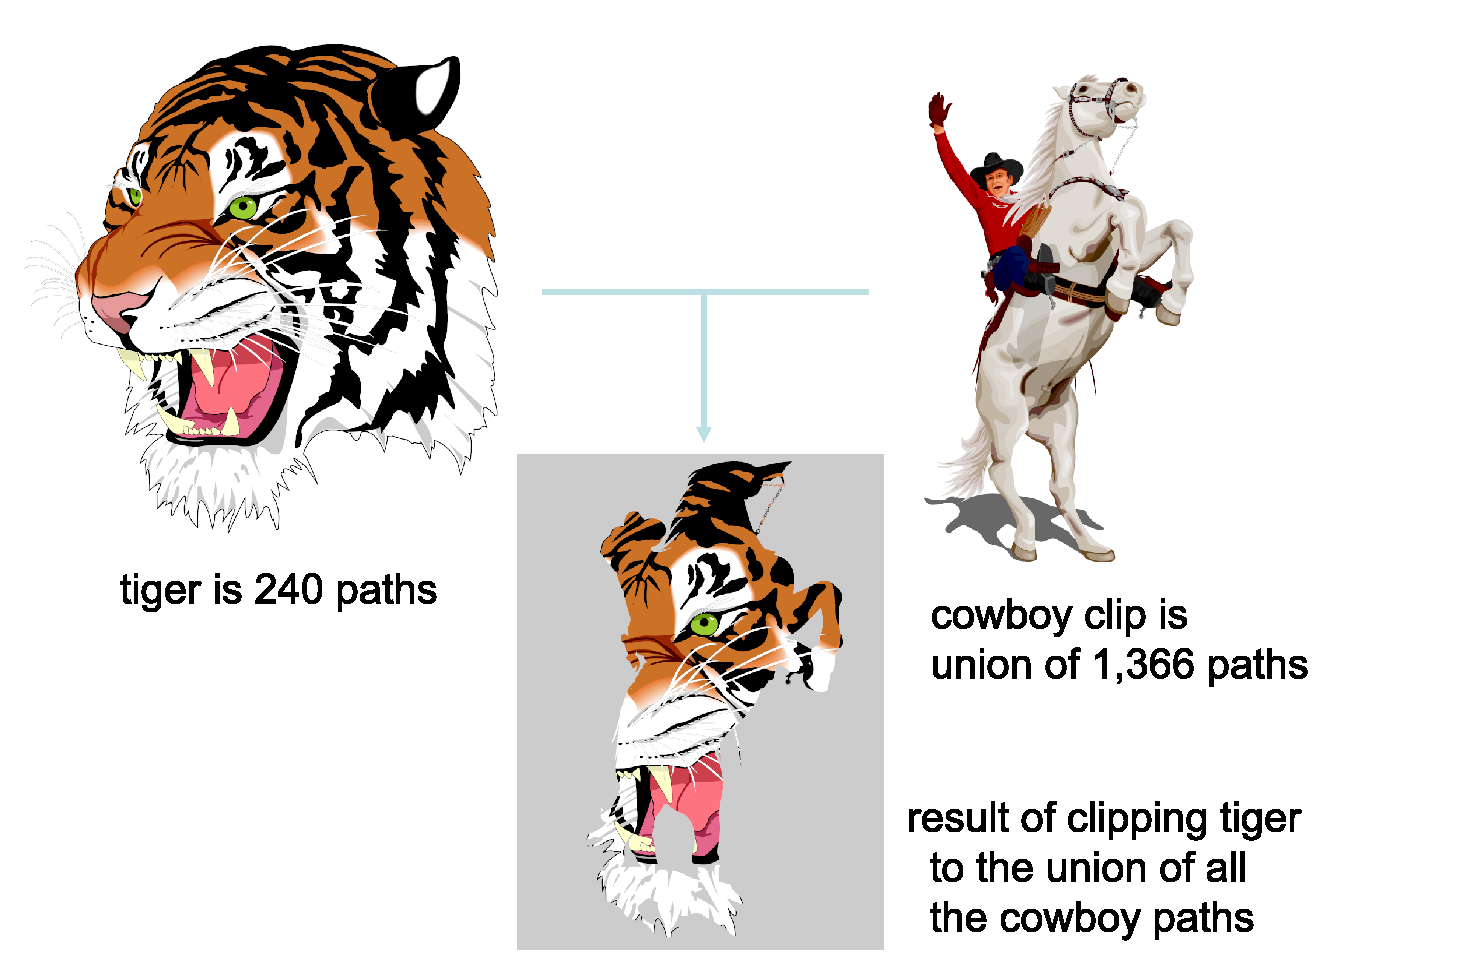
\includegraphics[width=\columnwidth]{clip_example.eps}}
  \center{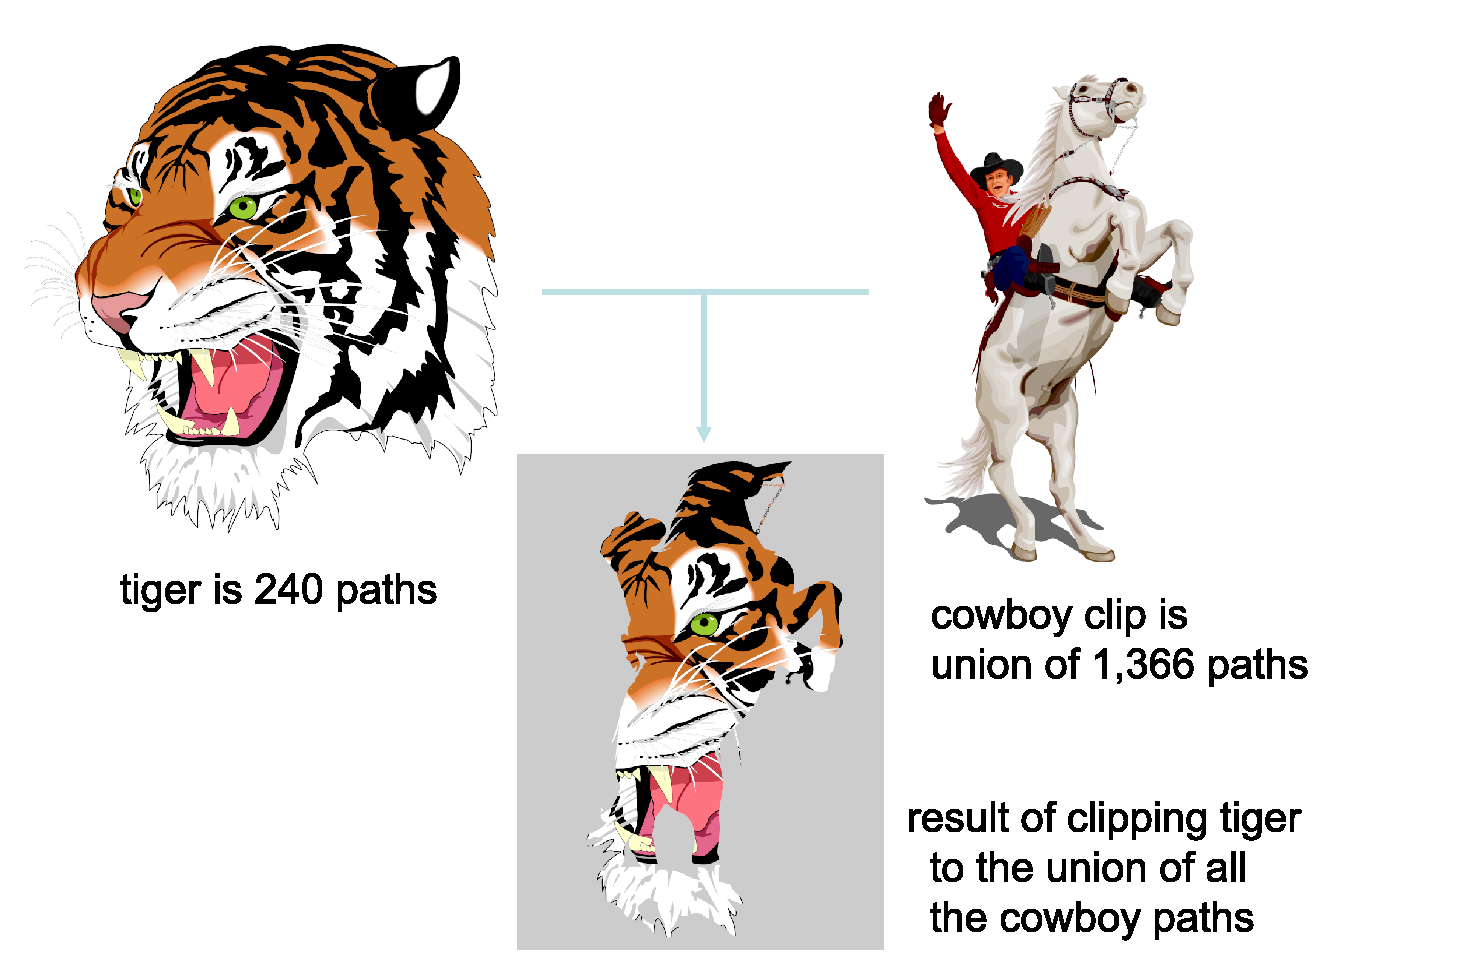
\includegraphics[width=3.6in]{clip_example.eps}}
  \caption{\label{fig:clip-example} Complex clipping scenario.
  Our approach: 8.69ms @ 1000x1000x16.  Cairo:  909ms @ 1000x1000.
  System: Core i7 + GeForce 560M GPU.}
\end{figure}

\subsection{Clipping to Arbitrary Paths}

All major path rendering standards support clipping a {\em draw}
path to the filled region of a {\em clip} path.
Our two-step ``stencil, then cover'' approach readily supports clipping
to arbitrary paths.  We briefly describe the process assuming an 8-bit
stencil buffer, initially cleared to zero:
%\vspace{-3pt}
\begin{enumerate}
  \item Stencil the clip path into the stencil buffer with a ``stencil
  fill'' operation.
  \item Perform a ``cover fill'' operation to coalesce the samples
  matching the fill rule so that the most-significant stencil bit is
  set and all the lower bits are cleared.  For example, if a sample's stencil
  value is non-zero, replace the stencil value with 0x80.
  This step updates only the stencil buffer (disable any color writes).
  \item Stencil the draw path into the stencil buffer with a ``stencil
  fill'' operation, but (a) modify only the bottom 7 bits of the stencil
  buffer, and (b) discard any rasterized samples without the topmost
  bit of the stencil buffer set.
  \item Perform a shaded ``cover'' operation on the draw path.  Update any
  color sample whose stencil value's bottom 7 bits are non-zero and
  zero the bottom 7 bits of the sample's stencil value.  Write shaded
  color samples during this step; due to the stencil configuration, only
  samples within both the clip and draw paths get shaded and updated.
  \item Finally to undo the clip path's stencil manipulation from step
  1, perform a ``cover'' operation on the clip path to reset the most
  significant stencil bit back to zero.
\end{enumerate}
Many variations on this approach are possible.  For example, steps
3 and 4 can be repeated for each path in a layered group of paths.
This avoids having to re-render the clip path for each and every path
in a group of paths.

Most standards allow nested clipping of paths to other paths.  Clever
manipulation of the stencil bit-planes allows such nested clipping.
Standards such as SVG allow for clipping to the union of an arbitrary
number of paths as shown in Figure \ref{fig:clip-example}.  Again, we can
accomplish this by clever use of stencil bit-planes and re-coalescing
coverage from different clip paths.
%  Conventional path clipping is the
%intersection of one path with another, but we can use the stencil buffer
%to compute the union, complement, or intersection of paths too.

\subsection{Painting}

What path rendering standards often call ``painting'' a filled or stroked
path is called shading in 3D graphics.  Our goal is to allow the full
generality of GPU-based programmable shading to be exposed when painting
paths.

During the cover step where a conservative bounding box or convex hull
is rendered to cover fully the stenciling of the path, the application
can configure arbitrary OpenGL shading.  This could be fixed-function
shading, assembly-level shaders, or shaders written in a high-level
language such as Cg or GLSL.

In conventional path rendering systems, linear and radial gradients are
a common form of paint for paths.  We note how straightforward radial
gradient paint can be implemented, including mipmapped filtering of the
lookup table accesses, with the following Cg shader:
%\vspace{-3pt}
\begin{lstlisting}
void radialFocalGradient(float3 str : TEXCOORD0.CENTROID,
                         float4 c   : COLOR.CENTROID,
                     out float4 color   : COLOR,
                 uniform sampler1D ramp : TEXUNIT0)
{
  color = c*tex1D(ramp, length(str.xy) + str.z);
}
\end{lstlisting}
%\vspace{-1em}
The texture coordinates needed for this shader can be generated as a
linear function of the path-space coordinate system.
Painting need not be limited to conventional types of path rendering
paint.  Arbitrary fragment shader processing can be performed during
the cover step (see Figure \ref{fig:bumpmap}).

\begin{figure}[tb]
  %\center{
\includegraphics[width=\columnwidth]{bumpmap.eps}}
  \center{
\includegraphics[width=3.3in]{bumpmap.eps}}
  \caption{\label{fig:bumpmap} Bump map shader applied to path rendered
  text, rendered from to different light positions, shown in yellow.}
\end{figure}

\subsection{Blending and Blend Modes}

OpenGL blending is sufficient for most path rendering where the
default path compositing operation is the ``over'' blend mode, assuming
pre-multiplied alpha.  Color writes during our cover step apply the
currently configured OpenGL blend state.
Modern GPUs also have efficient first-class support for blending in the
widely-used sRGB device color space.

%\subsubsection{sRGB Color Space}
%
%Modern GPUs have first-class support for blending in the sRGB color space.
%Such blending, while recognized as more correct for the broad variety of
%sRGB display devices, has been too expensive to justify for CPU-based
%path renderers.  With our approach, sRGB blending is easily configured
%with OpenGL and fast.

Sophisticated path rendering systems have additional blend modes
\cite{SVG-Compositing-Spec} beyond the standard Porter-Duff compositing
algebra \shortcite{Porter:1984:CDI:800031.808606}.  Digital artists are
familiar with these modes with names such as {\em ColorDodge}, {\em HardLight}, etc.
However GPU blending does not support these blend modes because they are
rare, complex, and not used by 3D graphics.  While some of these blend
modes can be simulated with multiple rendering passes, many of these modes
are impossible to construct from conventional GPU blending operations.

Our ``stencil, then cover'' approach makes it possible to implement
these blend modes despite their lack of direct GPU hardware support.
Normally, GPUs do not reliably support reading-as-a-texture a framebuffer
currently being rendered.  However a recent OpenGL extension called
{\tt NV\_texture\_barrier} \cite{TextureBarrier} provides a reliable memory
barrier under restrictive conditions.  A fragment shader must ensure
there is a single read and write for any particular pixel done from that
pixel's fragment shader instance.

The ``stencil, then cover'' approach provides precisely such a
``no double blending'' guarantee.  So by preceding each cover operation
(whether fill or stroke) with an OpenGL {\tt glTextureBarrierNV}  command and
reading the pixel's color value as a fetch to the framebuffer bound as
a texture, reliable programmable blending with the fragment shader is
possible.

